
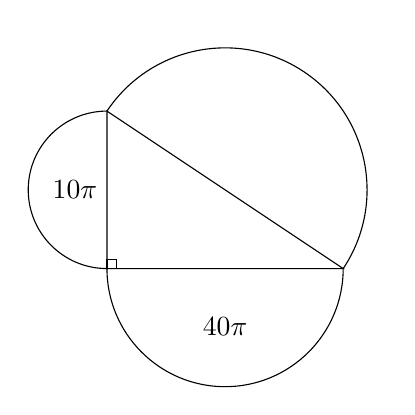
\begin{tikzpicture}
\draw(0,2)arc(90:270:1)(3,0)arc(360:180:1.5);
\draw(0,2)--(0,0)--(3,0)--cycle;
\draw(0,2)arc(146.31:-33.69:1.803);
\draw(0,1)node[anchor=east]{$10\pi$}(1.5,-0.5)node[anchor=north]{$40\pi$};
\draw(0,0)rectangle(0.12,0.12);
\end{tikzpicture}

Note: Diagram is \textbf{NOT} to scale.

Given the diagram above has a right triangle and three semicircles, and the labels above indicate the areas of two of the semicircles, find the total area of the figure in the diagram.



\ifsat
	\begin{enumerate}[label=\Alph*)]
		\item $25\pi+20$
		\item $50\pi+40$
		\item $100\pi+80$%
		\item $100\pi+160$
	\end{enumerate}
\else
\fi

\ifacteven
	\begin{enumerate}[label=\textbf{\Alph*.},itemsep=\fill,align=left]
		\setcounter{enumii}{5}
		\item $25\pi+20$
		\item $50\pi+40$
		\item $100\pi+80$%
		\addtocounter{enumii}{1}
		\item $100\pi+160$
		\item $200\pi+160$
	\end{enumerate}
\else
\fi

\ifactodd
	\begin{enumerate}[label=\textbf{\Alph*.},itemsep=\fill,align=left]
		\item $25\pi+20$
		\item $50\pi+40$
		\item $100\pi+80$%
		\item $100\pi+160$
		\item $200\pi+160$
	\end{enumerate}
\else
\fi

\ifgridin
 $100\pi+80$%
		
\else
\fi

